\documentclass[11pt]{article}
\usepackage[margin=0.9in]{geometry}
\usepackage{amsmath,amssymb,graphicx,booktabs,xcolor,array,tabularx,enumitem,float,caption}
\usepackage[hidelinks]{hyperref}
\graphicspath{{figures/}{../results/v2_samplerfix/}}
% generated by draft1/make_numbers.py -- do not edit
\newcommand{\NRegDossiers}{500}
\newcommand{\NRegTurns}{3000}
\newcommand{\NRegH}{186}
\newcommand{\NRegU}{342}
\newcommand{\NRegG}{2471}
\newcommand{\RegHpct}{6.2}
\newcommand{\RegGpct}{82.4}
\newcommand{\RegUpct}{11.4}
\newcommand{\NRegOnset}{135}
\newcommand{\NRegWrong}{64}
\newcommand{\NRegMissCode}{110}
\newcommand{\NRegInvented}{12}
\newcommand{\NClinDossiers}{300}
\newcommand{\NClinTurns}{1800}
\newcommand{\NClinH}{56}
\newcommand{\NClinU}{167}
\newcommand{\NClinG}{1577}
\newcommand{\ClinHpct}{3.1}
\newcommand{\ClinGpct}{87.6}
\newcommand{\ClinUpct}{9.3}
\newcommand{\NClinOnset}{44}
\newcommand{\NClinWrong}{24}
\newcommand{\NClinMissCode}{32}
\newcommand{\NClinInvented}{0}
\newcommand{\PilotVone}{0.0}
\newcommand{\PilotVtwo}{6.9}
\newcommand{\PrimRegL}{-0.034\,[-0.079,\,+0.015]}
\newcommand{\OnsetsRegL}{24}
\newcommand{\AucMzeroRegL}{0.755\,[0.640,\,0.859]}
\newcommand{\AucMoneRegL}{0.712\,[0.586,\,0.825]}
\newcommand{\AucMtwoRegL}{0.678\,[0.561,\,0.788]}
\newcommand{\AucMthreeRegL}{0.669\,[0.555,\,0.782]}
\newcommand{\AucMfourRegL}{0.836\,[0.752,\,0.908]}
\newcommand{\RhatMthreeRegL}{1.875}
\newcommand{\EssMthreeRegL}{6}
\newcommand{\RhatPreMthreeRegL}{2.345}
\newcommand{\EssPreMthreeRegL}{5}
\newcommand{\RhatMfourRegL}{1.663}
\newcommand{\EssMfourRegL}{6}
\newcommand{\RhatPreMfourRegL}{2.403}
\newcommand{\EssPreMfourRegL}{5}
\newcommand{\EvidRegL}{-0.033\,[-0.069,\,-0.008]}
\newcommand{\AmbRegL}{+0.001\,[-0.020,\,+0.033]}
\newcommand{\AmbPRegL}{0.52}
\newcommand{\HtwoPRegL}{0.0005}
\newcommand{\HtwoObsRegL}{27}
\newcommand{\HtwoNullRegL}{9.8}
\newcommand{\WithinPRegL}{0.159}
\newcommand{\WithinInfRegL}{35}
\newcommand{\BrierMthreeRegL}{-0.0003\,[-0.0007,\,+0.0001]}
\newcommand{\BrierBaseRegL}{+0.0004\,[-0.0004,\,+0.0011]}
\newcommand{\PrimRegX}{-0.008\,[-0.035,\,+0.021]}
\newcommand{\OnsetsRegX}{24}
\newcommand{\AucMzeroRegX}{0.755\,[0.640,\,0.859]}
\newcommand{\AucMoneRegX}{0.781\,[0.651,\,0.888]}
\newcommand{\AucMtwoRegX}{0.772\,[0.648,\,0.885]}
\newcommand{\AucMthreeRegX}{0.773\,[0.647,\,0.879]}
\newcommand{\AucMfourRegX}{0.820\,[0.716,\,0.906]}
\newcommand{\RhatMthreeRegX}{1.001}
\newcommand{\EssMthreeRegX}{2651}
\newcommand{\RhatPreMthreeRegX}{1.529}
\newcommand{\EssPreMthreeRegX}{7}
\newcommand{\RhatMfourRegX}{1.439}
\newcommand{\EssMfourRegX}{143}
\newcommand{\RhatPreMfourRegX}{1.047}
\newcommand{\EssPreMfourRegX}{105}
\newcommand{\EvidRegX}{-0.073\,[-0.129,\,-0.020]}
\newcommand{\AmbRegX}{+0.026\,[-0.023,\,+0.087]}
\newcommand{\AmbPRegX}{0.82}
\newcommand{\HtwoPRegX}{0.0005}
\newcommand{\HtwoObsRegX}{27}
\newcommand{\HtwoNullRegX}{9.8}
\newcommand{\WithinPRegX}{0.159}
\newcommand{\WithinInfRegX}{35}
\newcommand{\BrierMthreeRegX}{+0.0040\,[+0.0027,\,+0.0050]}
\newcommand{\BrierBaseRegX}{-0.0060\,[-0.0102,\,-0.0010]}
\newcommand{\PrimClinL}{-0.102\,[-0.208,\,-0.002]}
\newcommand{\OnsetsClinL}{8}
\newcommand{\AucMzeroClinL}{0.797\,[0.672,\,0.916]}
\newcommand{\AucMoneClinL}{0.844\,[0.778,\,0.912]}
\newcommand{\AucMtwoClinL}{0.742\,[0.591,\,0.885]}
\newcommand{\AucMthreeClinL}{0.810\,[0.657,\,0.948]}
\newcommand{\AucMfourClinL}{0.842\,[0.630,\,0.963]}
\newcommand{\RhatMthreeClinL}{1.590}
\newcommand{\EssMthreeClinL}{7}
\newcommand{\RhatPreMthreeClinL}{1.992}
\newcommand{\EssPreMthreeClinL}{5}
\newcommand{\RhatMfourClinL}{1.385}
\newcommand{\EssMfourClinL}{9}
\newcommand{\RhatPreMfourClinL}{1.426}
\newcommand{\EssPreMfourClinL}{8}
\newcommand{\EvidClinL}{-0.011\,[-0.057,\,+0.011]}
\newcommand{\AmbClinL}{+0.005\,[-0.007,\,+0.027]}
\newcommand{\AmbPClinL}{0.78}
\newcommand{\HtwoPClinL}{0.0020}
\newcommand{\HtwoObsClinL}{6}
\newcommand{\HtwoNullClinL}{1.5}
\newcommand{\WithinPClinL}{0.447}
\newcommand{\WithinInfClinL}{9}
\newcommand{\BrierMthreeClinL}{+0.0153\,[+0.0112,\,+0.0182]}
\newcommand{\BrierBaseClinL}{-0.0004\,[-0.0007,\,+0.0001]}
\newcommand{\PrimClinX}{-0.001\,[-0.004,\,+0.001]}
\newcommand{\OnsetsClinX}{8}
\newcommand{\AucMzeroClinX}{0.797\,[0.672,\,0.916]}
\newcommand{\AucMoneClinX}{0.844\,[0.732,\,0.943]}
\newcommand{\AucMtwoClinX}{0.843\,[0.730,\,0.942]}
\newcommand{\AucMthreeClinX}{0.826\,[0.624,\,0.963]}
\newcommand{\AucMfourClinX}{0.821\,[0.600,\,0.965]}
\newcommand{\RhatMthreeClinX}{1.001}
\newcommand{\EssMthreeClinX}{3053}
\newcommand{\RhatPreMthreeClinX}{1.723}
\newcommand{\EssPreMthreeClinX}{6}
\newcommand{\RhatMfourClinX}{1.386}
\newcommand{\EssMfourClinX}{146}
\newcommand{\RhatPreMfourClinX}{1.521}
\newcommand{\EssPreMfourClinX}{40}
\newcommand{\EvidClinX}{-0.092\,[-0.159,\,-0.024]}
\newcommand{\AmbClinX}{+0.053\,[+0.006,\,+0.124]}
\newcommand{\AmbPClinX}{0.99}
\newcommand{\HtwoPClinX}{0.0020}
\newcommand{\HtwoObsClinX}{6}
\newcommand{\HtwoNullClinX}{1.5}
\newcommand{\WithinPClinX}{0.447}
\newcommand{\WithinInfClinX}{9}
\newcommand{\BrierMthreeClinX}{-0.0032\,[-0.0038,\,-0.0024]}
\newcommand{\BrierBaseClinX}{-0.0075\,[-0.0106,\,-0.0037]}
\newcommand{\PHgivenH}{17.2}
\newcommand{\PHgivenNotH}{5.5}
\newcommand{\PosOnlyP}{2.3\times10^{-90}}
\newcommand{\DiffOnlyP}{0.463}
\newcommand{\CorrReg}{-0.120\,[-0.182,\,-0.070]}
\newcommand{\CorrBetterReg}{15}
\newcommand{\CorrWorseReg}{0}
\newcommand{\CorrSignReg}{6.1e-05}
\newcommand{\RegrReg}{-0.037\,[-0.093,\,+0.012]}
\newcommand{\RegrUReg}{+0.083}
\newcommand{\IvNReg}{121}
\newcommand{\OrigHReg}{14.5}
\newcommand{\CorrHReg}{2.5}
\newcommand{\CorrClin}{-0.098\,[-0.201,\,-0.028]}
\newcommand{\CorrBetterClin}{4}
\newcommand{\CorrWorseClin}{0}
\newcommand{\CorrSignClin}{0.12}
\newcommand{\RegrClin}{-0.024\,[-0.090,\,-0.001]}
\newcommand{\RegrUClin}{+0.041}
\newcommand{\IvNClin}{41}
\newcommand{\OrigHClin}{12.2}
\newcommand{\CorrHClin}{2.4}
\newcommand{\GuardSilentU}{2.3}
\newcommand{\GuardSilentG}{0.7}
\newcommand{\GuardHeld}{39}
\newcommand{\GuardHoldRate}{13.0}
\newcommand{\GuardPrec}{0.231}
\newcommand{\GuardRecall}{0.818}
\newcommand{\GuardHU}{2.3}
\newcommand{\GuardHG}{3.7}
\newcommand{\GuardPaired}{+0.013\,[-0.003,\,+0.037]}
\newcommand{\GuardMonCaught}{5}
\newcommand{\GuardMonTotal}{7}
\newcommand{\GuardMonHolds}{31}
\newcommand{\GuardThr}{0.091}
\newcommand{\GuardRegr}{131}
\newcommand{\GuardHHeld}{9}
\newcommand{\GuardHtot}{11}
\newcommand{\AtkClean}{6.1}
\newcommand{\AtkInj}{20.6}
\newcommand{\AtkPress}{8.6}
\newcommand{\AtkPressed}{12.3}
\newcommand{\AtkObey}{49}
\newcommand{\AtkAdopt}{11}
\newcommand{\AtkPressTurns}{146}
\newcommand{\AtkAucInj}{0.81}
\newcommand{\SbcPre}{0.003}
\newcommand{\SbcPost}{0.024}
\newcommand{\CovPre}{0.756}
\newcommand{\CovPost}{0.978}
\newcommand{\StarterFS}{41}
\newcommand{\StarterRhat}{1.71}
\newcommand{\StarterEss}{6}

\definecolor{navy}{HTML}{15334D}
\setlength{\parindent}{0pt}\setlength{\parskip}{6pt}
\captionsetup{font=small,labelfont=bf}
\newcommand{\fig}[3][\linewidth]{\begin{figure}[H]\centering\includegraphics[width=#1]{#2}\caption{#3}\end{figure}}
\begin{document}
\begin{titlepage}\color{navy}\vspace*{2.2cm}
{\Large\bfseries Academic Report --- draft 1}\\[1cm]
{\Huge\bfseries Hallucination Regime Lab}\\[.4cm]
{\LARGE Does conversation history help detect the first hallucination?\\ A Bayesian hidden-Markov study with a clinical guard application}\\[1.2cm]
{\large Nihar Narsana\\ MS Data Science --- Bayesian Inference and Modelling\\ University of Arizona}\\[1cm]
\color{black}
\begin{minipage}{.9\linewidth}\small
All numbers in this report are generated by \texttt{draft1/make\_numbers.py} from saved artifacts; Bayesian results come from the corrected-sampler re-runs (\texttt{results/v2\_samplerfix/}). Every patient, name and code is fictional. This is a research prototype, not a medical device.
\end{minipage}
\vfill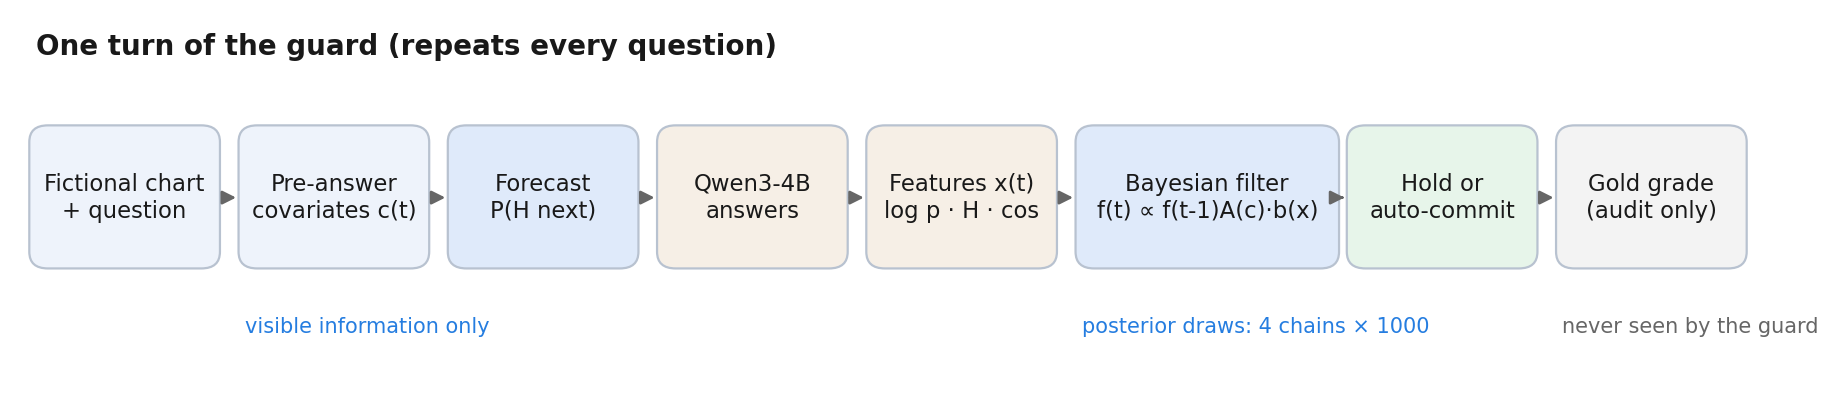
\includegraphics[width=\linewidth]{pipeline.png}
\end{titlepage}
\tableofcontents\newpage

\section{Executive summary}
We asked whether treating a language model's reliability as a \emph{hidden state that persists across turns} helps catch the first unsupported answer in a conversation. A local Qwen3-4B-Instruct model answered \NRegTurns{} registry questions and \NClinTurns{} clinical questions about fictional records. Every answer was graded against a gold record.

\begin{itemize}[leftmargin=*]
\item \textbf{History does not help detection.} The matched filter minus static onset-AUROC difference is \PrimRegL{} (registry) and \PrimClinL{} (clinical). Each answer's own features dominate.
\item \textbf{Errors cluster, but not provably through persistence.} The locked test finds clustering ($p=\HtwoPRegL$). An exact count-preserving null does not reject ($p=\WithinPRegL$), so the clustering is consistent with some dossiers simply being harder.
\item \textbf{Missing evidence is the clearest risk factor.} When the requested record is present, the risk of entering H changes by \EvidRegX{}.
\item \textbf{Errors snowball, and correcting them works (randomised).} Correcting the previous wrong answer lowered next-turn hallucination from \OrigHReg\% to \CorrHReg\% (\CorrReg).
\item \textbf{Application.} A Bayesian guard cut silent errors from \GuardSilentU\% to \GuardSilentG\% of answers on held-out clinical charts.
\item \textbf{Rigour.} An adversarial review found a sampler defect. After the fix, the exploratory homogeneous Bayesian HMM converges ($\widehat R=\RhatMthreeRegX$).
\end{itemize}

\section{Background and motivation: why this problem}
Hallucination in multi-turn use is not a sequence of independent events. Models commit to early assumptions and do not recover~\cite{laban}; errors propagate to later turns~\cite{halluhard}; and an early mistake can be elaborated into later ones~\cite{zhang}. In clinical record work, such as medication reconciliation, a wrong code that is \emph{silently} accepted is the dangerous outcome. A guard that flags risky answers before they are committed would therefore be useful, if it works.

\textbf{Why a hidden Markov model?} The quantity we care about, whether the model is currently answering from evidence, is not directly observable. We only see answers and their token statistics. An HMM models exactly this: a latent state $z_t$ that evolves by transitions and emits observations $x_t$. Its causal filter gives $P(z_t=H\mid x_{1:t})$ online, using every past turn. If states persist, the filter should beat any detector that looks at one answer in isolation.

\textbf{Why Bayesian?} Point estimates (EM) ignore parameter uncertainty and give no honest error bars on transition effects. A Bayesian treatment (i)~integrates over parameters when forecasting; (ii)~gives credible intervals for risk factors; (iii)~makes priors explicit, including a sticky prior that could \emph{manufacture} persistence, which we test as a sensitivity analysis; and (iv)~supports diagnostics (R-hat, ESS, SBC) that tell us when the inference cannot be trusted.

\section{Design decisions: what we chose and why}
\begin{table}[H]\centering\small
\begin{tabularx}{\linewidth}{p{.2\linewidth}p{.26\linewidth}X}\toprule
Decision & Chosen & Why (alternatives considered)\\\midrule
Model under test & Qwen3-4B-Instruct (Q4\_K\_M) via Ollama & Runs locally on a Mac and exposes top-20 log-probabilities. The \texttt{qwen3:4b} tag is a thinking model that ignored \texttt{think=false}, so the instruct tag was used. MLX was the original plan.\\
Task & Fictional dossiers with short codes & Gives \emph{independent} truth without an LLM judge; real data would need annotators.\\
Difficulty & Design v2 ($6\times5$, 2--6 hidden rows), frozen after the pilot & The v1 pilot produced almost no errors (\PilotVone\% H), too few onsets for any test. v2 gives \PilotVtwo\%.\\
Labels & G / U / H / P, deterministic grader & Keeps unwarranted abstention (U) distinct from hallucination (H)~\cite{kalai}. P (pending) marks ambiguous replies.\\
Features & log-prob, top-20 entropy, lexical cosine & Available for every token from the API. Semantic entropy needs repeated sampling; hidden-state probes need model internals~\cite{farquhar,kossen}.\\
Covariates & evidence, ambiguity, near-duplicates, turn & Computable \emph{before} the answer from visible information only, so they are valid inputs for a forecast.\\
Comparator & Matched static (same emissions) & The only way to isolate the value of \emph{history}. A negative control must reproduce it to $10^{-15}$.\\
Endpoint & First onset & Continued error turns would inflate a ``history helps'' result.\\
Sampler & FFBS-Gibbs with conjugate updates; MH for logits & Exact conditionals where conjugate. NUTS (PyMC) was unavailable on Python 3.14.\\
Exploratory model & log-surprisal transform, $M{=}1$ & Qwen's confidence is a near point mass, so two-component posteriors were multimodal. Labelled post hoc.\\
Decision rule & Bayes threshold $1/(1+10)$ & A missed wrong code is assumed 10$\times$ worse than an extra pharmacist check.\\\bottomrule
\end{tabularx}\caption{Main design decisions.}\end{table}

\section{How the system is used}
\subsection{Pipeline}
Fig.~\ref{fig:pipe} shows one turn of the guard. Before Qwen answers, the guard reads the visible chart and the question, computes covariates and forecasts the hallucination risk. After the answer it extracts features and updates the Bayesian filter, then either holds the answer for pharmacist verification or commits it. The gold grade is used \emph{only} to evaluate the guard.

\fig{pipeline.png}{The guard pipeline (one turn).\label{fig:pipe}}

\subsection{Commands and interface}
\begin{itemize}[leftmargin=*]
\item \texttt{collect.py} gathers resumable six-turn conversations from Ollama. \texttt{evaluate.py} fits M0--M4 and writes \texttt{report.json}. \texttt{intervene.py} runs the randomised branch experiment. \texttt{usecase\_clinical.py} runs the guard. \texttt{adversarial.py} runs the red-team and canary checks. \texttt{make\_report.py} generates every results text.
\item \texttt{example\_walkthrough.py --id 20003} prints one chart's chain update in the terminal.
\item \texttt{app.py} serves an interactive UI (Fig.~\ref{fig:ui1}): live runs against Qwen, replays, a live \emph{Hidden Markov chain} view, results and an explanation page.
\end{itemize}
\fig{ui_live.png}{Live run in the UI: patient chart, conversation, guard pipeline and risk timeline.\label{fig:ui1}}

\section{Worked example: one chart, step by step}
Chart 20003 is the lowest-ID held-out chart whose unguarded run contains an error; it was selected by that fixed rule. Table~\ref{tab:we} gives, for each turn, the covariates (evidence present / number of matching patients), the prior from the transitions, the answer, the evidence (normalised emission likelihood), the posterior, the guard decision and the independent grade. Probabilities are listed as G/U/H.

\begin{table}[H]\centering\scriptsize
\begin{tabularx}{\linewidth}{c>{\raggedright\arraybackslash}Xccccccc}\toprule
Turn & Question & Ev/Amb & Prior & Answer & Evidence & Posterior & Guard & Grade\\\midrule
1 & What is the imaging code for Greaves (born 1962)? & 1/2 & 0.71/0.07/0.22 & \texttt{VE6-33} & 0.00/0.00/1.00 & 0.00/0.00/1.00 & hold & H\\
2 & What is the ward code for Ilka Draycott? & 0/1 & 0.02/0.87/0.11 & \texttt{UNKNOWN} & 0.00/1.00/0.00 & 0.00/1.00/0.00 & commit & G\\
3 & What is the ward code for Garrow Fairbank? & 1/1 & 0.62/0.22/0.16 & \texttt{EE0-15} & 1.00/0.00/0.00 & 1.00/0.00/0.00 & commit & G\\
4 & What is the allergy code for Bennick Greaves? & 1/1 & 0.94/0.03/0.03 & \texttt{CB0-44} & 1.00/0.00/0.00 & 1.00/0.00/0.00 & commit & G\\
5 & What is the allergy code for Greaves (born 1962)? & 1/2 & 0.74/0.15/0.11 & \texttt{VE6-33} & 1.00/0.00/0.00 & 1.00/0.00/0.00 & commit & G\\
6 & What is that patient's medication code? & 0/1 & 0.01/0.88/0.11 & \texttt{UNKNOWN} & 0.00/1.00/0.00 & 0.00/1.00/0.00 & commit & G\\
\bottomrule\end{tabularx}
\caption{Worked example (corrected model; values recomputed from the saved run).\label{tab:we}}\end{table}


\textbf{Reading it.} On turn 1 the prior gives H only 0.22. Qwen then answers \texttt{VE6-33} with near-certainty. That is a real code, but it is Korvin Greaves's \emph{allergy} code, not his imaging code. Its features are evidence for H, the posterior moves to $P(H)=1.00$, and the guard holds the answer; the grade confirms H. On turn 2 the requested row is missing. The transitions route the prior to U (0.87), and the correct \texttt{UNKNOWN} keeps it there. On turn 5 the same string \texttt{VE6-33} is the correct allergy code and the posterior is G. The verdict depends on the evidence, not on the string. Fig.~\ref{fig:chain} shows the chain the UI builds live.

\fig{demo_markov_chain_final.png}{The Hidden Markov chain view for chart 20003: transition diagram $A(c)$, the trellis unrolled over turns (dashed rings are priors, filled circles posteriors), and the Bayes update strip.\label{fig:chain}}

\section{Priors}
Features are standardised on the training split, so the priors are on a unit scale. Fig.~\ref{fig:priors} plots each prior, together with the transition probability into H that the covariate priors imply.
\begin{table}[H]\centering\small
\begin{tabularx}{\linewidth}{p{.27\linewidth}p{.27\linewidth}X}\toprule
Parameter & Prior & Role and justification\\\midrule
Initial distribution $\pi$ & Dirichlet(1,1,1) & Uniform over the simplex; no state preferred at turn 1.\\
Transition rows $A_{i\cdot}$ (M3) & Dirichlet$(1+\kappa\mathbf 1[i{=}j])$, $\kappa=0$ & Neutral about persistence. The sticky values $\kappa=2,5$ are a \emph{sensitivity analysis}, because a sticky prior can manufacture persistence.\\
Mixture weights $w_j$ & Dirichlet(1,1) & Uniform split between a state's components.\\
Variances $v_{jmd}$ & InvGamma(3, 2) & Mean 1 on the standardised scale; keeps variances from collapsing onto point masses.\\
Means $\mu_{jmd}\mid v$ & $\mathcal N(0, v/0.5)$ & Marginally Student-$t$ with 6 df: weakly informative, heavy-tailed.\\
Logit intercepts $\alpha_{ij}$ (M4) & $\mathcal N(0,1.5^2)$ & Allows any baseline transition probability.\\
Covariate effects $\beta_{ij,k}$ (M4) & $\mathcal N(0,\sigma_k^2)$, $\sigma_k\sim$ HalfNormal(0.5) & Hierarchical shrinkage: unsupported effects are pulled toward 0.\\\bottomrule
\end{tabularx}\caption{Major priors.}\end{table}
\fig{priors.png}{Major priors and the prior predictive transition probability into H.\label{fig:priors}}

\section{Bayesian inference techniques used}
\subsection{Bayes' theorem for a latent-state model}
For parameters $\theta=(\pi,A,w,\mu,v[,\alpha,\beta,\sigma])$, hidden paths $z$, components $m$ and data $D$:
\[ p(\theta,z,m\mid D)\propto p(\theta)\,\prod_n \pi_{z_{n1}}\prod_{t\ge2} A_{z_{n,t-1}z_{nt}}(c_{nt})\prod_t w_{z_{nt}m_{nt}}\,\mathcal N(x_{nt};\mu_{z_{nt}m_{nt}},v_{z_{nt}m_{nt}}). \]
We sample from this joint posterior rather than maximising it.

\subsection{Exact forward filtering (the online detector)}
$q_t=f_{t-1}A(c_t)$ (prior), then $f_t(j)=b_j(x_t)q_t(j)/\sum_k b_k(x_t)q_k(t)$ (posterior). This is the guard's live computation. It is causal (it never uses future turns), and a canary test confirms that perturbing turns 4--6 leaves turns 1--3 unchanged. Computations are done in log space with log-sum-exp.

\subsection{Forward-filtering backward-sampling (FFBS)}
To sample whole paths jointly (not state by state, which mixes badly) we sample $z_T\sim f_T$ and then $p(z_t{=}i\mid z_{t+1}{=}j)\propto f_t(i)A_{ij}(c_{t+1})$. A test checks FFBS samples against exact path probabilities enumerated over $3^3$ paths.

\subsection{Conjugate Gibbs updates (M3)}
Given paths and components, counts give exact conditionals: $\pi\mid z\sim\mathrm{Dir}(1+N^{(0)})$; $A_{i\cdot}\mid z\sim\mathrm{Dir}(\alpha_{i\cdot}+N_{i\cdot})$; $w_j\sim\mathrm{Dir}(1+N_{j\cdot})$. For each component and feature, with $n$ points, mean $\bar x$ and sum of squares $S$:
\[ k_n=k_0+n,\; m_n=\tfrac{k_0m_0+n\bar x}{k_n},\; a_n=a_0+\tfrac n2,\; b_n=b_0+\tfrac S2+\tfrac{k_0n(\bar x-m_0)^2}{2k_n};\quad v\sim\mathrm{InvGamma}(a_n,b_n),\ \mu\sim\mathcal N(m_n,v/k_n). \]
The review found that $v$ was drawn with one Gamma variate shared across features. This is now fixed, with one independent draw per feature, and covered by a test.

\subsection{Metropolis-within-Gibbs (M4)}
Given the paths, each origin's logits form a multinomial-logistic regression with no conjugate prior. We use random-walk Metropolis--Hastings with a Laplace-shaped Gaussian proposal (inverse negative Hessian) adapted only during warm-up, plus an MH step on each $\log\sigma_k$ including the Jacobian. P\'olya--Gamma augmentation~\cite{holsclaw} would make this step exact Gibbs, and is listed as future work.

\subsection{EM baseline (not Bayesian)}
Baum--Welch maximises the likelihood (3 seeded starts). It provides the point-estimate comparator (M2), the matched static model (M1) and the reference used to align Bayesian draws.

\subsection{Label switching and state semantics}
The likelihood does not change if the state labels are permuted. We align each draw to the EM reference by its state-mean signature, and then map states to G/U/H using \emph{validation} labels only.

\subsection{Posterior prediction}
Risk is averaged over 200 posterior draws (a frozen ensemble). An importance-reweighted variant weights each draw by the likelihood of the prefix. Forecasts integrate $f_tA(c_{t+1})$ over the draws.

\subsection{Diagnostics and calibration of the inference}
Rank-normalised split $\widehat R$ and bulk/tail ESS~\cite{vehtari} use the gate $\widehat R\le1.01$, ESS $\ge400$; results from models that fail are labelled NONCONVERGED. Simulation-based calibration (SBC)~\cite{talts} draws parameters from the prior, simulates data, fits the model and checks that the ranks of the true values are uniform (Fig.~\ref{fig:sbc}). Posterior predictive checks compare lag-1 autocorrelation in observed and replicated data. Exact enumeration tests cover all $3^5$ paths.

\fig[.9\linewidth]{convergence.png}{Max $\widehat R$ before and after the variance-sampler fix.\label{fig:conv}}
\fig{sbc.png}{SBC rank histograms before and after the fix.\label{fig:sbc}}

\subsection{Bayesian decision theory and paired causal analysis}
With alert cost $C_{FP}$ and miss cost $C_{FN}$, holding when $P(H)>C_{FP}/(C_{FP}+C_{FN})$ minimises expected one-step loss. The randomised intervention uses matched seeds and is analysed with a Bayesian bootstrap over prefixes (Dirichlet weights), supplemented by exact sign tests and worst/best-case ITT bounds.

\section{Results}
\subsection{H1: does history help detection?}
No. M2 $-$ M1 is \PrimRegL{} (registry, locked), \PrimRegX{} (exploratory) and \PrimClinL{} (clinical). AUROCs (registry, exploratory): M1 \AucMoneRegX, M2 \AucMtwoRegX, M4 \AucMfourRegX{} (M4 fails the convergence gate).
\fig[.62\linewidth]{registry_exploratory/figures/roc_onset.png}{First-onset ROC curves (registry, exploratory, test).}
\fig[.75\linewidth]{registry_exploratory/figures/paired_auroc.png}{Paired AUROC differences with whole-dossier bootstrap intervals.}

\subsection{H2: do errors persist?}
The locked test finds clustering (\HtwoObsRegL{} vs.\ \HtwoNullRegL, $p=\HtwoPRegL$). After an H, the next answer was H in \PHgivenH\% of cases versus \PHgivenNotH\% otherwise. The exact within-dossier null that preserves each dossier's error count does not reject ($p=\WithinPRegL$ registry, $p=\WithinPClinL$ clinical; only \WithinInfRegL{} registry dossiers are informative). That null assumes exchangeable turn positions; a position-only control rejects ($p=\PosOnlyP$), whereas a difficulty-only control does not ($p=\DiffOnlyP$). Persistence beyond difficulty and turn effects is neither established nor excluded.
\fig[.75\linewidth]{h2_null.png}{Exact count-preserving null (registry).}

\subsection{H3: what raises the risk of hallucinating?}
Missing evidence: \EvidRegX{} (registry), \EvidClinX{} (clinical). Ambiguity: \AmbRegX. These are associations from M4, which has not converged, so they are provisional.
\fig[.8\linewidth]{registry_exploratory/figures/factor_forest.png}{Transition risk differences (M4).}

\subsection{H4: can the next answer be forecast?}
M3 parameter integration versus plug-in EM changes the Brier score by \BrierMthreeRegX{} (registry) and \BrierMthreeClinX{} (clinical). No forecaster beats the base rate (\BrierBaseRegX).

\subsection{H5: randomised correction}
On registry data, correction moved the next-turn H rate from \OrigHReg\% to \CorrHReg\% (\CorrReg, \CorrBetterReg/\CorrWorseReg{} prefixes better/worse, sign test $p=\CorrSignReg$). On clinical data the effect was \CorrClin{}, but it rests on few discordant prefixes. Re-grounding: \RegrReg{}, with unwarranted \texttt{UNKNOWN} up by \RegrUReg.
\fig[.75\linewidth]{registry/figures/intervention.png}{Intervention contrasts (registry).}

\subsection{Application and red team}
The guard (threshold \GuardThr) held \GuardHHeld/\GuardHtot{} errors with a hold rate of \GuardHoldRate\% and cut silent errors from \GuardSilentU\% to \GuardSilentG\%. Re-grounding did not help (\GuardPaired), and monitor-only is recommended. Under indirect prompt injection the H rate went from \AtkClean\% to \AtkInj\%; under sycophancy pressure, to \AtkPressed\% on pressured turns.
\fig[.7\linewidth]{usecase/figures/usecase.png}{Clinical guard outcomes.}

\section{Validation and the adversarial review}
Every finding was reproduced independently before any change was made. A change was implemented only on unanimous acceptance after independent reproduction, under explicit anti-reward-hacking rules. The review's key outcomes were:
\begin{itemize}[leftmargin=*]
\item The variance-sampler defect was fixed and all Bayesian fits were re-run with identical configuration. EM results reproduced exactly, and M3 now passes the convergence gate (Fig.~\ref{fig:conv}).
\item The H2 headline was weakened to match the evidence.
\item Convergence claims were corrected, and every unconverged result is now labelled.
\item Provenance digests were added to the red-team results, and the guard's threshold policy is now stated explicitly.
\item The predecessor starter was audited: its thresholds caused \StarterFS\% clean false stops and its sampler had $\widehat R=\StarterRhat$, ESS \StarterEss.
\end{itemize}

\section{Limitations and future work}
\begin{itemize}[leftmargin=*]
\item The task is fictional, uses short codes and a single 4B checkpoint, and measures entropy through a top-20 proxy.
\item The clinical test split has only \OnsetsClinL{} onsets.
\item M4 and all two-component fits fail the convergence gate. Future work: P\'olya--Gamma or independence-MH samplers with a pre-registered SBC plan.
\item The state posterior is not a calibrated error probability. Future work: calibration and conformal risk control~\cite{mohri}.
\item H2 needs a model that adjusts jointly for dossier difficulty and turn effects.
\end{itemize}

\appendix
\section{Reproduction}
\begin{verbatim}
python3 verify.py                                   # offline tests
python3 evaluate.py --dir runs/registry --out results/registry
python3 evaluate.py --dir runs/registry --out results/registry_exploratory \
        --transform log_surprisal --M 1
python3 intervene.py --dir runs/registry --out results/registry
python3 usecase_clinical.py --results results/v2_samplerfix/clinical_exploratory
python3 app.py                                      # interactive UI
python3 draft1/make_numbers.py && python3 draft1/make_figures.py
\end{verbatim}
\fig{ui_results.png}{Research-results view of the UI.}

\begin{thebibliography}{99}\small
\bibitem{laban} P.~Laban \emph{et al.}, ``LLMs get lost in multi-turn conversation,'' arXiv:2505.06120, 2025.
\bibitem{halluhard} ``HalluHard,'' arXiv:2602.01031, 2026.
\bibitem{zhang} M.~Zhang \emph{et al.}, ``How language model hallucinations can snowball,'' ICML 2024.
\bibitem{kalai} A.~T. Kalai \emph{et al.}, ``Why language models hallucinate,'' arXiv:2509.04664, 2025.
\bibitem{farquhar} S.~Farquhar \emph{et al.}, ``Detecting hallucinations \ldots\ semantic entropy,'' \emph{Nature}, 2024.
\bibitem{kossen} J.~Kossen \emph{et al.}, ``Semantic entropy probes,'' arXiv:2406.15927, 2024.
\bibitem{holsclaw} T.~Holsclaw \emph{et al.}, \emph{Ann. Appl. Stat.}, 2017.
\bibitem{vehtari} A.~Vehtari \emph{et al.}, ``Rank-normalization \ldots\ $\widehat R$,'' \emph{Bayesian Analysis}, 2021.
\bibitem{talts} S.~Talts \emph{et al.}, ``Simulation-based calibration,'' arXiv:1804.06788, 2018.
\bibitem{mohri} C.~Mohri, T.~Hashimoto, ``Conformal factuality guarantees,'' ICML 2024.
\end{thebibliography}
\end{document}
